\documentclass[11pt]{IEEEtran}
\usepackage[brazilian]{babel}
\usepackage[utf8]{inputenc}
\usepackage[T1]{fontenc}
\usepackage{float}
\usepackage{graphicx}
\usepackage{caption}

\captionsetup[table]{skip=10pt}

\sloppy

\title{Programação Paralela\\ Trabalho III}

\author{Giovanni Cupertino, Matthias Nunes, \IEEEmembership{Usuário pp12820}}

\begin{document}

\maketitle

\section{Introdução}

	O objetivo do trabalho é desenvolver uma solução que ordene diversos vetores
	utilizando o algoritmo Quick Sort.  Os vetores contém cem mil elementos e
	são, no total, dez mil vetores que estão na ordem inversa de valores indo de
	noventa e nove mil novecentos e noventa e nove na primeira posição até zero
	na ultima posição.  Para a abordagem paralela do trabalho, utilizou-se uma
	implementação híbrida utilizando as ferramentas MPI\@ e OpenMP. Para esta 
	abordagem temos um dos processos como mestre, que é responsável por mandar 
	mensagens com os vetores a serem ordenados pelos nós do cluster e reorganizar
	os vetores nas suas posições originais na estrutura. Os outros processos 
	(escravos) recebem os vetores, os ordenam e devolvem ao mestre utilizando o 
	OpenMP para a exploração do paralelismo com memória compartilhada dentro do nó.

\section{Análise dos Resultados Obtidos}

	É possível observar que o tempo de resposta para dois
	processos é maior que quando executado sequencialmente, isso ocorre pelo
	fato de que só temos um processo realizando a ordenação e o outro como
	mestre, havendo um tempo extra principalmente pela troca de mensagens entre
	os dois, como pode ser visto na tabela~\ref{result_table}.

	\begin{table}[H]
		\centering
		\scalebox{0.8}{
			\begin{tabular}{c|r|r|r|r}
				Núcleos & Tempo de Execução(s) & Speed-Up & Speed-Up Ideal & Eficiência \\
				\hline
				1 & 6,59000 & 1,00 & 1 & 1,00 \\
				\hline
				2 & 10,31665 & 0,63877 & 2 & 0,31939 \\
				\hline
				4 & 3,77560 & 1,74542 & 4 & 0,43635 \\
				\hline
				5 & 2,51584 & 2,61941 & 5 & 0,52388 \\
				\hline
				8 & 2,63324 & 2,50262 & 8 & 0,31283 \\
				\hline
				11 & 2,26792 & 2,90575 & 11 & 0,26416 \\
				\hline
				12 & 2,31676 & 2,84449 & 12 & 0,23704 \\
				\hline
				16 & 2,38038 & 2,76846 & 16 & 0,17303 \\
				\hline
				20 & 2,70099 & 2,43985 & 20 & 0,12199 \\
				\hline
				24 & 2,58161 & 2,55267 & 24 & 0,10636 \\
				\hline
				28 & 2,53986 & 2,59463 & 28 & 0,09267 \\
				\hline
				32 & 2,69780 & 2,44273 & 32 & 0,07634 \\
			\end{tabular}
		}
		\caption{Resultados obtidos}
		\label{result_table}
	\end{table}

	\begin{figure}[H]
		\centering
		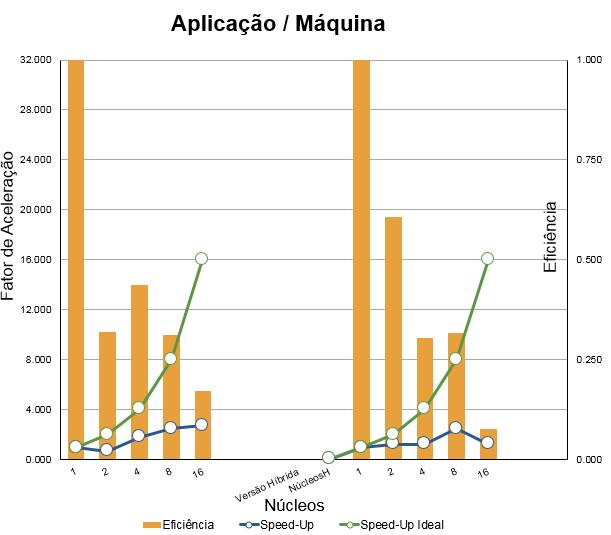
\includegraphics[width=88mm]{doc/graph.png}
		\caption{Gráfico gerado a partir da tabela}
		\label{fig_graph}
	\end{figure}

	Essas pequenas diferenças, como a troca de mensagens, a reorganização dos
	vetores nas suas posições inicias e a comunicação entre os 2 nós utilizados
	também reduzem a eficiência e criam diferenças entre o speed-up ideal e o
	real. Devido a velocidade do algoritmo de ordenação o tempo para realizar a
	tarefa depois de cinco processos permaneceu bastante semelhante, já que os
	escravos terminam a sua tarefa antes mesmo do mestre conseguir enviar uma
	nova para todos os processos que estão solicitando.  Algumas alternativas
	para maior utilização dos núcleos, para os casos com mais de cinco, seriam
	possuir mais de um mestre permitindo maior distribuição de vetores aos
	escravos(cada um controlando escravos diferentes e passando os vetores
	quando lhes forem requeridos) e a utilização de um algoritmo de ordenação
	mais lento que proporcionaria mais tempo ao mestre para distribuir vetores
	aos escravos, ou seja, antes que tivesse novas requisições.

	O fato de se estar utilizando dois nós e a biblioteca MPI permite um
	balanceamento da carga igualitário dos processos nos núcleos físicos ($8$ em
	cada uma das máquinas com capacidade de simular $16$ threads). Mesmo
	utilizando capacidades acima de dezesseis processos
	(\emph{hyper-threading}), não foi possível observar melhoras significativas
	nos tempos de execução e por consequência no speed-up e na eficiência.

\section{Dificuldades Encontradas}

	Não foram encontradas dificuldades na implementação desse trabalho, nem na
	utilização da biblioteca MPI\@.

\end{document}

